\documentclass[parskip=full, a4paper]{scrreprt}

%%% PACKAGES %%%

% add unicode support and use german as language
\usepackage[utf8]{inputenc}
\usepackage[ngerman]{babel}

% Use Helvetica as font
\usepackage[scaled]{helvet}
\renewcommand\familydefault{\sfdefault}
\usepackage[T1]{fontenc}

% Better tables
\usepackage{tabularx}

% Better enumerisation env
\usepackage{enumitem}

% Use graphics
\usepackage{graphicx}

% Have subfigures and captions
\usepackage{subcaption}

% Be able to include PDFs in the file
\usepackage{pdfpages}

% Have custom abstract heading
\usepackage{abstract}

% Need a list of equation
\usepackage{tocloft}
\usepackage{ragged2e}

% Better equation environment
\usepackage{amsmath}

% Symbols for most SI units
\usepackage{siunitx}

\usepackage{csquotes}

% Clickable Links to Websites and chapters
\usepackage{hyperref}

% Change page rotation
\usepackage{pdflscape}

% Symbols like checkmark
\usepackage{amssymb}
\usepackage{pifont}

\usepackage[absolute]{textpos}

% Glossary, hyperref, babel, polyglossia, inputenc, fontenc must be loaded before this package if they are used
\usepackage{glossaries}
% Redefine the quote charachter as we are using ngerman
\GlsSetQuote{+}
% Define the usage of an acronym, Abbreviation (Abbr.), next usage: The Abbr. of ...
\setacronymstyle{long-short}

% Bibliography & citing
\usepackage[
backend=biber,
style=apa,
bibstyle=apa,
citestyle=apa,
sortlocale=de_DE
]{biblatex}
\addbibresource{Referenzen.bib}
\DeclareLanguageMapping{ngerman}{ngerman-apa}

%%% TOC Header
\addto\captionsngerman{
	\renewcommand{\contentsname}{Traktanden}
}

%%% Not clearpage before chapter
\usepackage{etoolbox}
\makeatletter
\patchcmd{\scr@startchapter}{\if@openright\cleardoublepage\else\clearpage\fi}{}{}{}
\makeatother
%%% DOCUMENT %%%

\begin{document}
\begin{titlepage}
\vspace*{2.5cm}
\noindent
\Huge{\textbf{Sitzungsprotokoll SprintReview}} \\
\noindent
\Large{19.03.2019, Rotkreuz}\\
\vfill
\noindent
\large{Author: Dane Wicki}\\
\noindent
\large{Datum: \today}\\
\end{titlepage}

\noindent
\begin{tabularx}{\textwidth}{XXl}
\hline \\
\multicolumn{3}{l}{\Large{\textbf{SprintReview  Bachelorarbeit}}}\\
\multicolumn{3}{l}{Suche von mit RFID ausgerüsteten Einzelexemplaren} \\ \\
\hline
	Freitag, & & Hochschule Luzern \\
	19. März 2019 & 08:00 Uhr bis 09:30 Uhr & Raum 41.412 - 8, Rotkreuz \\
\hline \\
\hline
Besprechungsart & SprintReview & \\
\hline
Besprechungsleiter & Pascal Baumann & \\
\hline
Protokollführer & Dane Wicki & \\
\hline
Teilnehmer & Mike Märki & \\ & Pascal Baumann & \\ & Dane Wicki & \\
\hline
Abwesend & Prof. Martin Jud & \\
\hline
\end{tabularx}

	\noindent

\tableofcontents
\chapter{Protokoll und Aufgabenstellung}

Es wurde kurz das Protokoll der letzten auf Sitzung gegengefragt ob dieses so korrekt sei. Herr Märki bestätigte, die Korrektheit des Protokolls.

Pascal Baumann legte Herr Märki die konkrete Aufgabenstellung zur Unterschrift bereit. Herr Märki unterzeichnete diese.

\chapter{Präsentation der Sprint Resultate}

Herr Wicki begann mit dem Vorzeigen des Ablaufes der Sprints.
Es wurde erklärt, dass ein Sprint 2 Wochen dauert, und all 4 Wochen ein Meeting mit Herr Märki angestrebt wird.

\chapter{Präsentation Konzept 1}

Herr Wicki stellte das Ziel des 1. Konzeptes vor, dass ein bestimmtes, bekanntes Exemplar im Hochregallager deplatziert wurde. Er führte weiter an, dass ein solcher Fall eintreten könnte, würde ein Exemplar von der Speicherbiliothek bestellt und dieses nicht im entsprechenden Behälter vorhanden wäre. Das Exemplar muss dementsprechend im Hochregallager zu finden sein.
Weiter sagte er, dass in diesem Konzept ein Spezieller Behälter entwickelt werden, welche ins Hochregallager gesendet werden kann. Weiter führte er an, dass nur genau ein Exemplar abgesucht werden kann, da diese Methodik Geschwindigkeitsvorteile bietet. Herr Märke fragte ob der Grund für diese Geschwindigkeitsvorteile niedergeschrieben wurden. Herr Wicki bestätigte, dass dies im Konzept beschrieben ist.

Herr Baumann erklärte darauf noch den Suchalgorithmus von RFID HF. Er erklärte, dass bei RFID HF ein Detection Prevention Algorithmus zum Einsatz komme. Dieser würde die Tags mittels einer Maskierung anfragen. Trifft diese Maske auf einen Tag zu würde dieser Antworten. Trifft er auf mehrere zu detektiert das Lesegerät eine Kollision und definiert die Eingabemaske genauer, bis nur ein Tag dieser Maske entspricht. Weiter führte Herr Baumann auf, dass sofern die ID eines Tags bekannt sei der Algorithmus nicht gebraucht werden würde, da nur ein Tag antworten kann. Dies würde zu einem schnelleren auffinden des Tags führen.

Herr Märki fragte nach, ob es eine Möglichkeit gäbe in den Raum zu fragen, welche Tags vorhanden seien, Herr Baumann erklärte, dass dies nicht möglich sei.

Herr Wicki führte nochmals nach, dass nur ein Tag auf einmal gelesen werden können, ansonsten empfängt man nicht spezifizierbare Daten.
Herr Wicki erklärte, dass das im Konzept Spezifizierte Lesemodul mit dem Gebrauch des Prävention Algorithmus 50 Tags in der Sekunde lesen könne, weshalb es für einen Tag nicht länger gehen kann als 1/50 Sekunden.

Herr Märki fragt ob dieser Algorithmus spezifiziert sei. Herr Baumann erwiderte, dass diese in der ISO Norm genau spezifiziert sind.
Weiter fragte Herr Märki ob nicht Mehrere Tags aufs mal gelesen werden könne, Herr Wicki erwiederte, dass der Roboter eine Geschwindigkeit von maximal 24m/s haben dürfte, wenn nur ein Tag gelesen werden würde. Der Roboter bewege sich jedoch nur 6m/s womit bei dieser geringeren Geschwindigkeit 3 Tags auf einmal abgesucht werden können.
Herr Märki führte noch an, dass es sehr aufwändig ist in der Gasse nach einem Exemplar zu suchen, daher wäre es nützlich könne man gleich mehrere Tags absuchen.

Herr Wicki erklärte anschliessend, dass in diesem Konzept 2 Suchmodi zum Einsatz kämen. Dies aus dem Grund, dass RFID HF eine Theoretische Maximale Distanz von 1m beträgt. Die Distanz im Hochregallager beträgt jedoch 1.2m, da zwei Behälter jeweils hintereinander gelagert werden. Es ist in diesem Konzept dementsprechend nicht möglich mit der Vorbeifahrt die Tags der hinteren Box herauszulesen. Daher kämen zwei Suchmodi zum Einsatz, der Erste würde eine Oberflächliche Suche starten, welche lediglich den vorderen Behälter nach dem Tag absucht. Somit könnte eine Abdeckung von ca. 50\% gewährleistet werden.
Weiter führte Herr Wicki auf, dass für den ersten Suchmodus dieses Konzeptes mehrere Antennen um die Rechte wie auch die Linke Gasse simultan auslesen zu können. Die Dauer dieses Suchmodus Beträge gut drei Minuten pro Gasse.

Herr Märki stellte anschliessend die Frage, ob der Roboter auch in der Höhe die Behälter absucht. Herr Wicki verwies auf die Graphik \ref{fig:antennenpos}, auf welcher aufgezeigt wird, dass bei Position 2 und 3 die Obere wie auch die Untere Reihe zur Selben Zeit gelesen werden sollen um so nur jede 3 Reihe durchfahren zu müssen. Dies müsse jedoch in einem Proof of Concept evaluiert werden.
Herr Märki stellte fest, dass die Positionierung der Pos. 3 Direkt auf das Metall des Roboters ausgerichtet wäre. Herr Baumann erwiederte, dass ein Vorteil von RFID HF gegenüber RFID UHF in der geringen Störung durch Metall liegt.

\begin{figure}
	\centering
	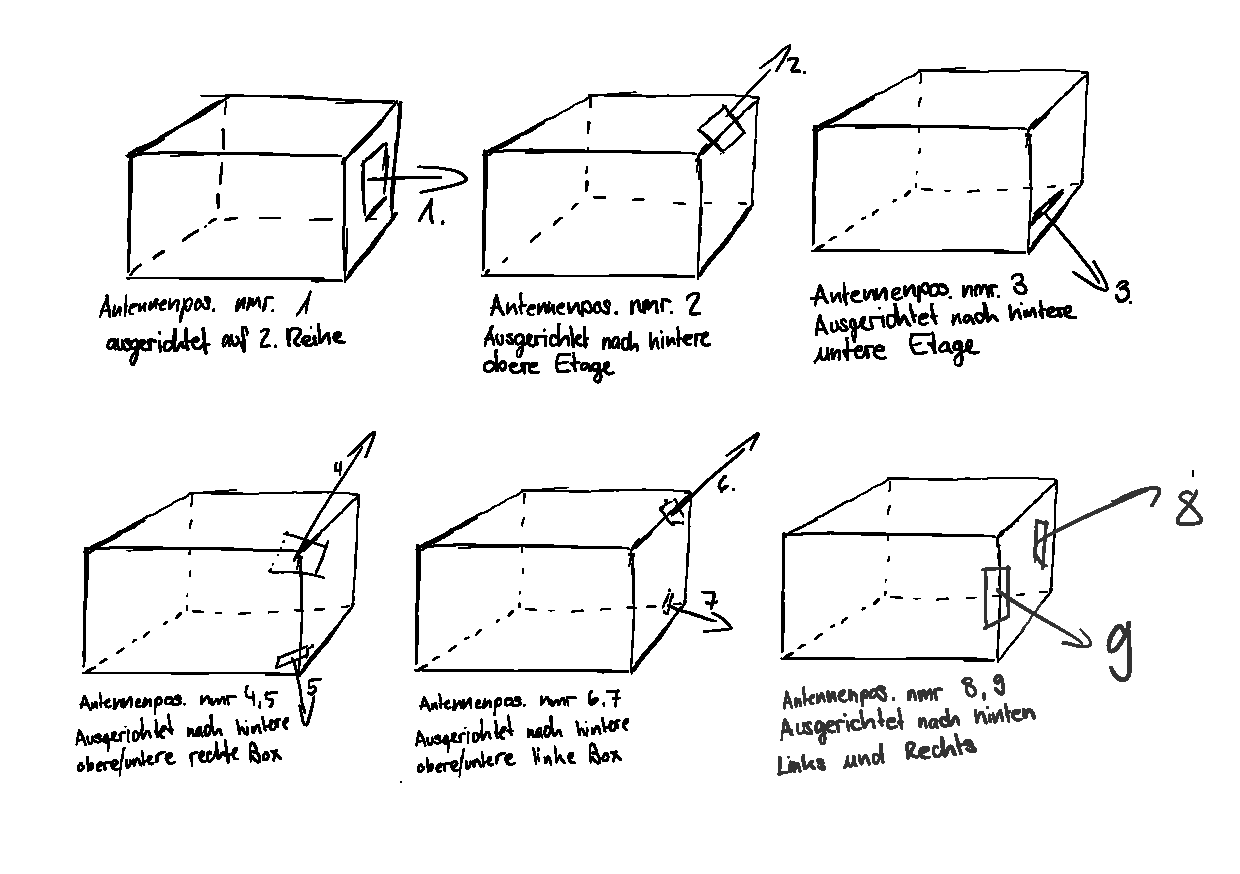
\includegraphics[keepaspectratio, width=0.8\linewidth]{images/Konzept_1_Drawings3.pdf}
	\caption{Positionen der Antennen}
	\label{fig:antennenpos}
\end{figure}

Herr Wicki erklärte weiter, dass beim Suchmodus Nummer zwei die Boxen der vorderen Reihe ausgetauscht werden würden. Dazu müsste gemäss diesen Konzeptes die bestehende Verwaltungssoftware erweitert werden. Damit der Roboter autonom die Boxen absuchen könnte. Herr Wicki führte auf, dass dieser Suchvorgang ca. 4h dauert pro Reihe, sofern der Austausch 2er Boxen nicht länger als 10s betrage. Sobald der Lesebehälter die Position eines Vorderen Behälters eingenommen hat sollen gleich alle neun hinteren Behälter ausgelesen werden gemäss den Antennenpositionen auf \ref{fig:antennenpos}. Somit kann eine Geschwindigkeitssteigerung des Faktors 9 erreicht werden. Der Vorteil dieses Konzeptes läge in der Abdeckung von bis zu 100\%. Herr Wicki fasste zusammen, dass die Störung durch Metall wie auch die Interferencen mehrere Antennen noch in einem Proof of Concept eruiert werden müssen. Und eben diese Faktoren sehr grosses Fehlerpotential in diesem Konzept aufweisen.

Herr Wicki zeigte nochmals die Antennenpositionen auf der Graphik \ref{fig:antennenpos}. Dabei sollen die Positionen 4 - 6 Lediglich für den zweiten Suchmodus verwendet werden.
Herr Märki fragte darauf, ob beide Reihen gelesen werden können. Herr Wicki bestätigte dies, dass bei Suchmodus zwei Beide Reihen gelesen werden könnten.
Herr Baumann Zweichnete anschliessend eine Graphik (wie Graphik \ref{fig:boxenposition}), welche die Position der Box veranschaulicht. Dabei erklärte er, dass die 9 Hinteren 9 Boxen simultan gelesen werden.

\begin{figure}
	\centering
	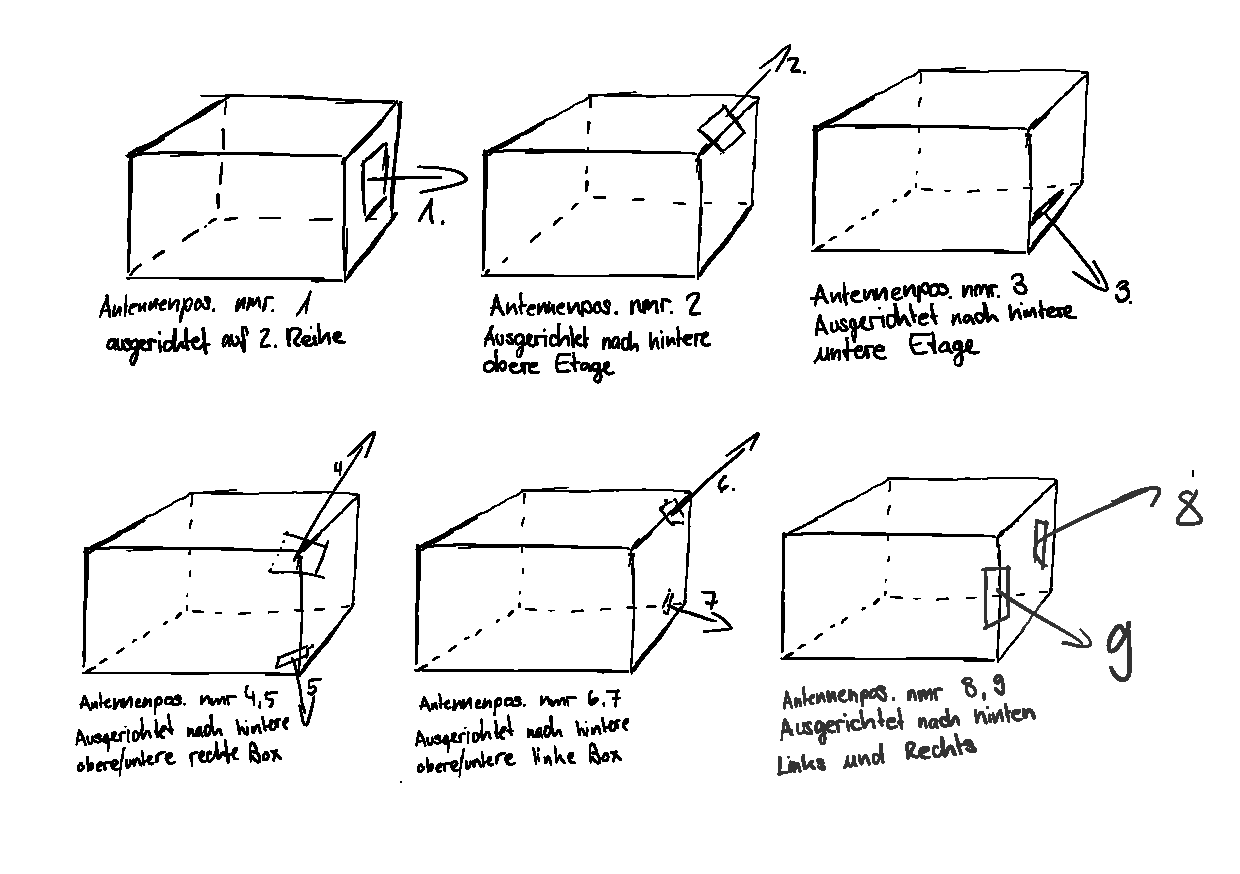
\includegraphics[keepaspectratio, width=0.8\linewidth]{images/Konzept_1_Drawings3.pdf}
	\caption{Positionen der Antennen}
	\label{fig:antennenpos}
\end{figure}

Herr Märki wies dabei noch darauf hin, dass die Positionen der Behälter nicht fix ist, sie also über den Tag an neue Positionen gelangen können. Herr Wicki erklärte, dass diese nur beim Zeitpunkt der Auslese relevant sei, da anschliessend mit der Behälter ID gearbeitet werden sollen.
Her Märki fragte anschliessen, dass man so jedoch wissen müsse, welcher Behälter sich auf einer Bestimmten Position befinden würde. Herr Wicki wie Herr Baumann bestätigten dies.
Herr Wicki führte weiter an, dass bei der Erweiterung der Verwaltungssoftware zudem noch so erweitert werden würde, dass dieser in irgendwelcher form mitgeteilt werden kann, dass der Lesebehälter mit einem Behälter an einem Spezifischen Platz ausgetauscht werden würde. Herr Baumann merkte an, dass eine Manuelle Eingabe der Fahrt nach jedem Behälteraustausch nicht Praktikabel wäre. Herr Märki fasste zusammen, dass die Behälterposition flüchtig seien.

Weiter fügte Herr Märki an, dass die Verwaltungssoftware eine Meldung erhalten sollte, sofern das Exemplar gefunden werden würde und dann die Suche beendet werden müsse. Herr Wicki merkte an, dass dies über die Steuersoftware gemacht werden würde, und deshalb deren Änderung auch im Konzept stehe. Er führte weiter aus, dass eine Schnittstelle zur Steuersoftware mitteilen können müsste, welche Box von Roboter angefahren wird und was die Position des Roboters im Moment ist. Herr Märki merkte an, dass eine Steuerung des Roboters aus dem Inneren der Box wahrscheinlich schwierig sei, und dies von extern gemacht werden müsste. Was im Moment schon möglich ist, ist das Schicken des Roboters an eine spezifische Position. Inwiefern dies dann angepasst werden müsste, wäre sicher nicht Teil der Arbeit. Für Herrn Märki schon ein Gewinn wäre eine funktionierende Suchbox welche die Exemplare lokalisieren könnte.

Herr Wicki erklärte wie die Kommunikation angedacht sei. Insbesondere, dass auf dem Arbeitsplatzcomputer beim Umschlagplatz für Exemplare eine Software laufen würde, auf der der momentane Fortschritt angezeigt würde, und falls das Exemplar gefunden worden ist, in welchen Behältern das Exemplar sein könnte, eventuell geordnet nach Wahrscheinlichkeit. Er merkte an, dass dafür eben die Position des Roboters bekannt sein müsse, und dies ein Knackpunkt dieses Konzept sei. Herr Märki äusserte Bedenken darüber, ob diese Voraussetzung wirklich umsetzbar sei. Da der Roboter nur ein Fahrauftrag bekomme und daher die Position des Roboters gar nicht zu jeder Zeit bekannt sein müsse.
Herr Wicki merkte an dass bei diesem Konzept sehr viele Unbekannten existieren, wie die Anpassung der Steuersoftware, welche man zuerst eruieren müsste. Herr Märki wies darauf hin, das im schlimmsten Fall der Roboter auch manuell durch die Gassen geschickt werden könnte. Und die Auffindung eines Exemplars audiovisuell, durch eine Signallampe oder Sirene dargestellt werden könnte. Herr Baumann merkte an, dass dies natürlich nur für die Behälter gerade neben der Gasse möglich sei, da die Reichweite einfach zu kurz sei um bis zum Zweiten Behälter durchdringen zu können.
Herr Märki merkte danach an, dass beim zweiten Suchmodus die Position eigentlich bekannt sei, da ein spezifischer Behälter ausgetauscht würde, und sonst der Behälter über die Tags in der Umgebung bestimmt werden könnte. Herr Baumann erwiderte daraufhin, dass dies bedingt, dass genügend Exemplare mit RFID ausgestattet sind und in der Umgebung aufzufinden wären. Herr Wicki merkte an, dass dann auch wieder die Geschwindigkeit für das Auslesen mehrerer Tags relevant werden würde.
Herr Märki fragte ob es eine Signalstärke des Tags gäbe. Herr Baumann erwiderte dass dies nicht bekannt ist, und erklärte daraufhin die Funktionsweise des Lesers in Kürze.
Herr Märki fasste zusammen, das schon ein Suchbehälter welcher den Suchmodus Eins umsetzt helfen würde.

Herr Wicki präsentierte daraufhin was für Kosten für die Behälter anfallen würde. Herr Baumann erwiderte, dass dies Demopreise seien, welche bei einem effektiven Produkt eventuell nicht mehr gelten.
Herr Märki merkte an, dass es eventuell Vertreiber von Geräten dieses Herstellers in der Schweiz gäbe, und man diese nach Leihgeräten anfragen könnte.
Danach ging Herr Wicki auf die Kosten der Softwareentwicklung für die Steuerungssoftware ein und die Annahmen die dafür getroffen wurden. Als Anmerkung bemerkte Herr Märki, dass es ein Nachtventilationsprogramm gibt, bei dem der Roboter ohne einen Behälter zu entnehmen durch die Gassen fährt. Er vermutet daher, dass eine solche Schnittstelle realisierbar sein müsste. Aber ein Gassenwechsel wahrscheinlich nicht so einfach zu Realisieren sei.
Auch bemerkte Herr Wicki, dass die finale Umsetzung dann in einer weiteren BDA geschehen würde.
Danach nannte Herr Wicki die Vorteile dieses Konzept. Dies wären das Auffinden von Exemplaren, welche mit RFID markiert sind, und das autonome Arbeiten des Roboters.
Herr Märki bemerkte auch, dass er sich vorstellen könnte, dass das Suchprogramm dann vom Lieferanten des Roboters implementiert würde, und in diesem Projekt rein der Behälter entwickelt würde, welcher eine Rückmeldung an den Roboter sendet. Herr Wicki erwiderte, dass es vorstellbar sein könnte, dass man dies über WLAN bewerkstelligt, da im Suchbehälter sowieso ein kleiner Computer vorgesehen sei.
Herr Wicki merkte an, dass ein Nachteil dieses Konzeptes auch die im 1000 CHF Bereich liegende Batterie sei. Auf Rückfrage wieso dies so teuer sei, erwiderte er, dass es Hauptsächlich an der langen, unabhängigen (also nicht am Stromnetz angeschlossen) Laufzeit des Suchbehälters und der Entladung des Akkus liege. Der grösste Nachteil aus Sicht des Projektteams seien die Kosten und Unbekannten welche mit diesem Konzept zusammenhängen.
Ein grosses Problem seien die langen Distanzen, die Überbrückt werden müssen, gemäss Berechnungen im Konzept seien dies bi 977mm. Ob dies unter Realbedingungen erreichbar ist, sei fraglich und müsse getestet werden.

\chapter{Präsentation Konzept 2}
Herr Baumann erklärte die Grobidee des zweiten Konzeptes, dass es im Prozess des Einlagerns eine weiter Prüfung durchgeführt würde, nämlich alles Tags identifiziert und erkennt wenn ein Tag nicht in den zu prüfenden Behälter gehört.

Er erklärte, dass bedingt durch die Lesegeschwindigkeit von mehreren Tags (deren 50 pro Sekunde) der Behälter stationär sein müsste, oder sich zumindest nur langsam bewegt. Dafür wurden in der Erarbeitung des Konzeptes vier Positionen identifiziert. Dies wären bei der Arbeitstation selber, in der Eckpartie, auf der Waage und im Lift. Bei der ersten Position wären eventuell andere störende Exemplare in der Umgebung, und bei der Letzteren wäre der Behälter schon kurz vor dem Einlagern. Er schlussfolgerte daher, das die Eckpartie oder bei der Waage die Positionierung am gescheitesten sei. Da bei diesen ausgewählten Positionen der Behälter nicht stillstehe, existieren noch die Unbekannten wie schnell die Tags effektiv ausgelesen werden können und ob dies auch während einer Bewegung geschehen kann. Herr Märki erwiderte, dass nicht alle Tags ausgelesen werden müssten. Auf die Antwort das mindestens ein fehlplatziertes Exemplar immer gefunden werden müsse, erwiderte Herr Märki dass dies ja sowieso nicht immer gegeben sei.
Herr Baumann erklärte danach die Positionierung der Antenne, da in dem zweiten Konzept bis jetzt nur eine angenommen sei. Die Position der Antenne sei über dem Förderband als eine Art Tor angedacht. Falls das Förderband und deren Elektronik das Auslesen nicht beeinträchtige, sei es auch eine Möglichkeit die Antenne unter dem Förderband anzubringen. Dies seien aber ebenfalls Unbekannte die in einem weiteren Schritt genauer beleuchtet werden müssten.

Herr Märki merkte an, dass die Antenne eventuell besser an der Seite montiert werden müsste, da die RFID Tags der Exemplare vertikal stehen und nicht liegen. Herr Baumann stimmte dem zu, und bemerkte dass Fragen über die Ausrichtung der Tags zum Magnetfeld in einer Evaluation auf jeden Fall beantwortet werden müssten.
Danach ging Herr Baumann auf die Signalisierung ein. Eine Möglichkeit sei das automatisierte Aussortieren des Behälters, welches aber eine Schnittstelle zur Förderbandsteuersoftware voraussetze. Eine Alternative wäre ein audiovisuelles Signal in Form einer Drehlampe und Sirene, welche den Mitarbeiter eine Unstimmigkeit mitteilen würde. Zwei weitere Konzepte wären Benachrichtigungen auf den Computer der Mitarbeiter oder einfach ein Log indem Behälter mit Unstimmigkeiten eingetragen würden.
Herr Märki antwortete, dass für ein Proof Of Concept ein optisches Signal, denkbar in Form einer Signallampe, reichen würde. Bei einer produktiven Lösung müsste der Behälter auf jeden Fall aussortiert werden. Herr Baumann erwiderte, dass das Projektteam die Annahme hatten, das eine Aussortierung möglich sein müsste, die Frage wäre aber ob die Implementation dieser Funktionalität von ihnen oder dem Hersteller des Lagerverwaltungssystem umgesetzt werden müsste.

Weiter müsste der Behälter selber identifiziert werden, dies kann entweder über einen weiteren Barcodescanner oder über die Identifizierung aller Tags und anschliessendem Analysieren der Behälterzugehörigkeit realisiert werden. Die letztere Lösung bedingt jedoch, dass mindestens zwei weitere RFID Tags neben dem Zielexemplar im Behälter vorhanden sind.
Herr Märki fügte an, dass für den Proof of Concept sogar nur ein Bericht für die Signalisierung reichen würde, da sie dann Zeit hätten, diesen Behälter wieder zurückzuholen. Für die technische Seite der Identifikation, wäre für Herrn Märki auch denkbar, dass die Lösung rein nur die Identifikation der Tags übernimmt und eine Liste an das Lagerverwaltungssystem übermittelt. Dieses müsste diese Information dann mit der internen Datenbank abgleichen. Herr Baumann merkte an, dass dies für ihre Lösung von Vorteil sei, da dann weniger Rechenaufwand auf der Seite des kleinen Computers der Lösung gemacht werden müsste. Herr Märki fasste zusammen, dass er für einen Proof Of Concept rein ein Auslesen und Bericht über den Inhalt des Behälters machen würde. Der Barcodeleser wäre für Ihn auch eine Möglichkeit, er schätzt dies für einen Proof Of Concept jedoch zu aufwändig ein.
Herr Baumann ging danach auf die Kosten dieses Konzepts ein. Dort seien die Unbekannten rein die Anzahl der Antennen, welche in einem weiteren Schritt identifiziert werden müssten.
Herr Baumann erklärte dass die Hersteller FEIG, Metrotec und Siemens für Leihgeräte angefragt worden seien, aber neben Feig von allen noch keine Rückmeldung erhalten worden seien. Herr Märki erklärte, dass er in der Woche danach auf einem Bibliothekskongress sei und die Augen offenhalten würde.
Herr Wicki erwiderte, dass die Kosten für dieses Konzept im Moment noch Hoch angesetzt sei, da für die Berechnungsgrundlage die Long Range Antenne genommen wurde. Es gäbe für kürzere Reichweiten auch andere Hersteller und günstigere Antennen. Herr Märki sieht das Problem vor allem darin, dass selbst für einen Proof of Concept Kosten anfallen, und wünscht dass sich das Projektteam noch nach anderen Möglichkeiten umschauen soll.

Herr Baumann ging dann auf die Vorteile ein, welche vor allem sind, dass dieses Konzept direkt in den Prozess integriert sei und keine Änderungen an den bestehenden Systemen gemacht werden müssen. Der Nachteil liege darin, dass bereits eingelagerte Exemplare nicht gefunden werden können. Weiter seien in den identifizierten Anforderungen eine Auslesung von 200 Tags spezifiziert, dies würde in etwa vier Sekunden gebrauchen. Es wäre daher in einer nächsten Phase wichtig, diese Fragen zu analysieren und das Konzept kritisch zu evaluieren. Herr Märki merkte an, dass es nicht möglich sei, den Behälter vier Sekunden lang stehen zu lassen. Herr Baumann merkte an, dass dem Projektteam dies bewusst sei, dass man aber schon in der Abbremsbewegung des Behälters anfange auszulesen. Es müsse also einfach mindestens ein Teil des Behälters im Lesebereich sein. Es sei auch die Frage ob wirklich 200 Tags in einem Behälter seien, worauf Herr Märki erwiderte dass dies üblicherweise nicht der Fall sei, und er der Meinung ist, dass 50 Tags die Regel sei. Herr Märki sagte auch, dass ein weiteres Problem der Position bei der Waage sei, dass noch andere Behälter in der Nähe in Bewegung seien welche eventuell Lesefehler verursachen können. Er identifizierte daher die Position beim Lift als eine bessere Position, da diese in der Umgebung abgeschirmt sei. Herr Baumann erwiderte darauf, dass beim Lift eventuell Störung durch Elektromagnetismus der Motoren passieren könnte. Herr Märki präzisierte danach, dass man sich vorstellen kann, das Konzept nicht im Lift zu realisieren sondern davor. Dort seien die Behälter auf den Lift am Warten und stünden still. Dort hätte man die Möglichkeit direkt zwei Behälter auszulesen, welche stillstünden. Das Problem sei eventuell, dass beide Behälter auf eine Leseabfrage antworten würden.
% 58:00
\end{document}